\section{Whose values enter technological change?}

Creative destruction expands opportunity while reorganizing work, distribution, and
legitimate coordination \citep{schumpeter1942capitalism,aghion1992model,mokyr2002gifts,nobel2025}.
Language models increasingly frame these trade-offs in decision support and agent
workflows. Even with a fixed application and prompt, a new release can change which
responses it presents as typical for a named country. We call agreement with observed
response distributions \emph{country-conditioned survey representation}; this construct
does not measure latent model preference, normative advice, or culture itself.

Prior evidence confirms that model choice and prompting matter. WorldValuesBench reports
normalized-W1 success from 11.1\% to 75.0\% across four systems
\citep{zhao2024worldvaluesbench}; Tao et al. find country-prompt gains in 71--81\% of
countries or territories for later GPT versions \citep{tao2024cultural}. Their different
protocols cannot identify the effect of one release under a fixed design.

We therefore ask which aspects of country-conditioned representation improve, persist, or
worsen when the survey target and elicitation protocol remain fixed. EthosGPT follows the
same survey evidence from item fidelity to country profiles and cross-country geometry,
using paired inference at each scale. An exact finite-pool identity separates run-varying
error from mismatch shared before agent interaction, and a declared sensitivity analysis
relates the changes to creative-destruction margins for opportunity, adjustment, and
coordination. Figure~\ref{fig:spatial-maps} connects the prior benchmarks, this comparison,
and the economic questions it opens.

Countries are survey units rather than uniform cultures, repeated generations do not
constitute an agent society, and English country labels cannot establish local validity.
These boundaries motivate multilingual, within-country, and community-led research on
whether changes in survey representation become consequential in local use. We release
data and code on GitHub.

\begin{figure}[t]
  \centering
  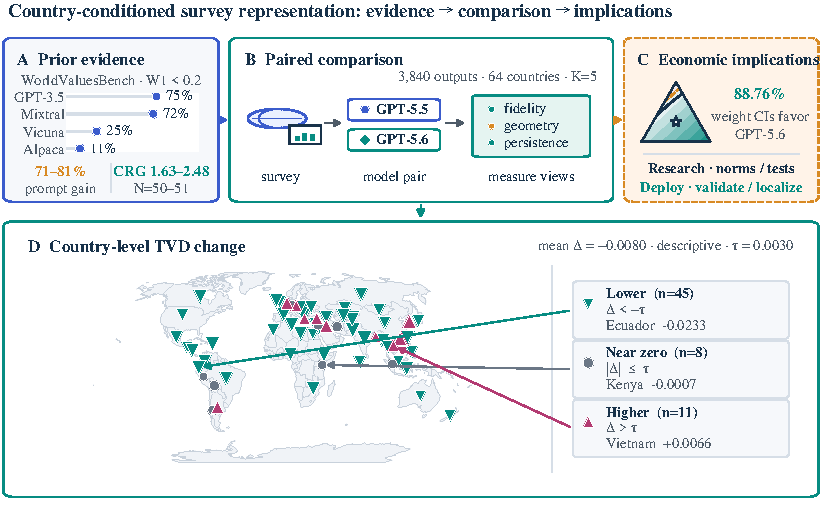
\includegraphics[width=\linewidth]{figs/fig1_spatial_story.pdf}
  \caption{From earlier benchmarks to a release-specific comparison. \textbf{A},
  protocol-separated evidence from prior studies. \textbf{B}, the paired
  survey--model measurement design. \textbf{C}, the continuous creative-destruction
  weight surface and the research and deployment questions it motivates.
  \textbf{D}, the 64-country TVD change; Ecuador, Kenya, and Vietnam illustrate lower,
  near-zero, and higher error under $\tau=0.1\max|\Delta|=0.0030$; labels and rules sit
  outside the map. Solid marks report observed evidence, whereas dashed connectors mark
  questions for future study. The map is descriptive and provides no evidence of
  diffusion or culturally uniform regions.}
  \label{fig:spatial-maps}
\end{figure}
